\documentclass{article}

\usepackage[%
    left=0.5in,%
    right=0.5in,%
    top=0.5in,%
    bottom=0.5in,%
]{geometry}%
\usepackage{minitoc}
\usepackage{multicol}
\usepackage{graphicx}
\usepackage{fixltx2e}
\usepackage{listings}
\usepackage{color}
\usepackage{hyperref}
    \hypersetup{ colorlinks = true, linkcolor = blue }
\usepackage{blindtext}
\definecolor{lightgray}{gray}{0.9}
\graphicspath{ {./} }

\newcommand{\inlinecode}[2]{\colorbox{lightgray}{\lstinline
[language=#1]$#2$}}
\newcommand{\worddef}[1]{\hyperref[sec:reference]{\textit{#1}}}

\begin{document}

\tableofcontents

\newpage

\section{Schwartz	algorithm}
\begin{flushleft}
Consider a tree-operation (e.g. +-reduce) performed by $P$ parallel processes on $n$ data items, where $P < n$:
\begin{itemize}
  \item The tree should connect the P processes, rather than the n data items
  \item i.e. each process should compute a local result on $n / P$ data items, which are then combined by a P-leaf tree 
  \item Rather than, e.g., creating a tree of n-1 processes each combining one pair of values 
\end{itemize}
This will minimise \textbf{communication, coordination and overhead} (e.g. thread creation and multiplexing) but still have maximal parallelism if \texttt{P = number of processors}
\end{flushleft}

\subsection{Discussion}
\begin{itemize}
  \item Essentially this is an application of the locality rule to treebased algorithms 
  \item It is a general strategy that is assumed to be used for, e.g., \textit{reduce and scan} operations 
  \item Typically the most important aspect is \textbf{having each process performed a balanced share} of the computation locally
  \item When P is relatively small (e.g. multicore computer) there will be \textbf{little observable difference} between sequential (critical section) and tree-based coordination between processes
\end{itemize}

\section{Reduce}
\begin{itemize}
  \item Reduce combines a set of values to produce a single value – E.g. count3s sum of counts across threads 
  \item It is almost always necessary at some point to compare or combine values from different threads, e.g. to summarise the computation or control its execution
  \item Some computers even have hardware support for reduction, e.g. BlueGene/L
  \item Assumed to be implemented using a Schwartz-style algorithm, i.e.
  \begin{itemize}
    \item Each thread combines a portion of the data to produce its own value
    \item Values from each thread are then \textbf{combined in a tree} to produce the global value 
  \end{itemize}
\end{itemize}

\begin{center}
  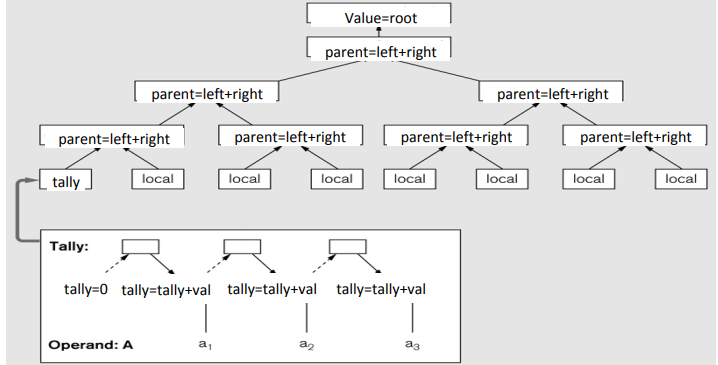
\includegraphics[scale=0.5]{reduce.png}
\end{center}

\subsection{Generalised Reduce}
\begin{itemize}
  \item For simple reductions (as in OpenMP) there is a single summary value which is the same type as one data item
  \item E.g. +-reduce or max-reduce, reduces an array of floats (data items) to one float (summary value) 
  \item Reduce can be generalised: 
  \item The intermediate or tally value calculated by each thread can be a different type from the data items
  \item The global summary value can be a different type from the tally values
  \item They need not be single values, e.g. they could be compound values or array
\end{itemize}

\subsection{Implementing	Generalised	Reduce}
\begin{itemize}
  \item \verb!init()! – initialise a thread’s tally value 
  \item \verb!accum(tally,val)! – combine a single data value with a thread’s running tally
  \item \verb!combine(left,right)! – combine left and right tally values 
  \item \verb!reduceGen(root)! – convert the root tally value to the global summary value
\end{itemize}

\begin{center}
  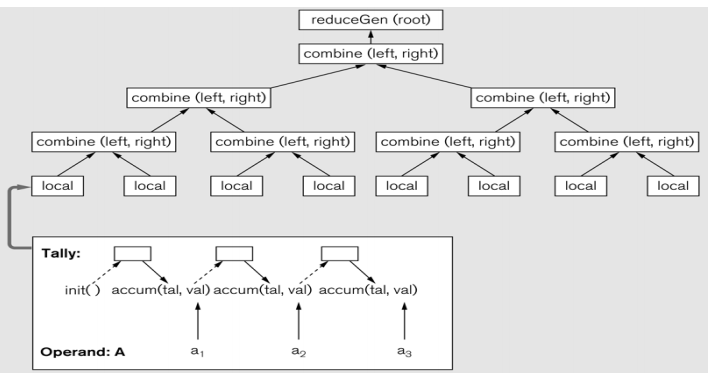
\includegraphics[scale=0.5]{reduce_combine.png}
\end{center}

\section{Scan}
\begin{flushleft}
Parallel scan is another common parallel operation for calculating \textbf{local information} that depends on \textbf{non-local information}. Specifically that depends on information on the “left” of each value. Requires two passes:
\begin{itemize}
  \item One upward pass, like reduce, calculating intermediate values 
  \item One downward pass, combining and distributing intermediate values back down the tree to the individual threads 
  \item In this case, the sum of all values to the left of the left-most child of a node
\end{itemize}
\end{flushleft}

\subsection{Key points}
\begin{itemize}
  \item Many parallel computations can be decomposed into blocks of independent parallel computation on local data interspersed with reduce and scan operations
  \item Reduce and scan have efficient parallel implementations that scale well to large number of processors
  \item Some thought may be required to see how a global operation can be solved as a generalised reduce or scan
\end{itemize}

\section{Static work allocation}
\begin{itemize}
  \item Consider the common case where we have a 1- or 2-dimensional array of data to distribute between some set of processes for some parallel computation 
  \item Our general approach is to \textbf{maximise locality}, so in most cases we will allocate contiguous portions of the data structure to each process
  \item The values operated on by each process will therefore be close to each other, and separate from values allocated to other processes 
  \item For a 1-D array this will probably just be blocks on consecutive indices (as in the count3s examples)
\end{itemize}

\subsection{Work allocation for 2D arrays}
\begin{itemize}
  \item Work allocation for 2D arrays, fften each calculation will depend on \textbf{several neighbouring values} in the array – E.g. calculating the average value of that item and its neighbours, and other stencil computations 
  \item In this case it is usually best to allocate \textbf{square-like blocks} of values to each process – More of the values needed are therefore local to the process.
  \item And for bigger arrays the difference grows as $O(n/2)$ vs $O(n)$
\end{itemize}

\subsection{Overlap regions}
\begin{itemize}
  \item The block allocation still requires some \textbf{non-local references} 
  \item It will usually be better to explicitly \textbf{fetch and cache} the required overlap regions first, and then perform the computation entirely locally 
  \item Batching communication like this also tends to reduce overhead, esp. on disjoint memory machines 
  \item If the computation is iterative then threads will need to synchronise at each step, e.g. with a barrier
\end{itemize}

\subsection{Block cyclic allocations}
\begin{itemize}
  \item In some algorithms work is \textbf{not proportional} to the amount of data. E.g. some iterative algorithms require different numbers of iterations for different parts of the data
  \item In this case – giving each process a single large contiguous block of data may result in \textbf{poor load balancing}
  \item It is better to allocate each process many \textbf{smaller blocks of data spread across the entire array}. Typically using a block-cyclic allocation…
\end{itemize}

\begin{center}
  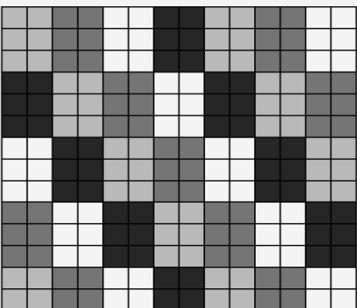
\includegraphics[scale=0.5]{block_alloc.png}
\end{center}

\begin{flushleft}
Each process is still allocated data in blocks, rather than rows, to reduce \textbf{non-local memory access}. But each process is allocated many different blocks, so that hopefully on average each process ends up with a comparable amount of work to do, even if some blocks take longer than others.
\end{flushleft}

\section{Dynamic work allocation}
\begin{flushleft}
A static work allocation may not always be possible or efficient, e.g.
\begin{itemize}
  \item Data references may be irregular, as in a graph or mesh
  \item The amount of work required for each data item may be very variable and unpredictable 
  \item E.g. with an adaptive algorithm, that changes its behaviour depending on the results so far
  \item Work may continue to arrive while the program executes. e.g. an online server
\end{itemize}
\end{flushleft}

\subsection{Work queues}
\begin{flushleft}
\begin{itemize}
  \item The work queue itself is a shared data structure that holds the definitions of the currently unallocated tasks 
  \item E.g. blocks of data to be processed 
  \item The simplest possible work queue is a first-in first-out (FIFO) list of tasks
  \item The task description in the work queue should be as small as possible (to reduce overhead)
  \item Tasks should be of suitable granularity – Too many small tasks will increase overhead; too few large tasks will result in idle processors 
  \item For a large system multiple parallel work queues should be used – to prevent the work queue becoming a serial bottleneck
\end{itemize}
\end{flushleft}

\pagebreak
\section*{Reference section} \label{sec:reference}
\begin{description}
	\item[placeholder] \hfill \\
\end{description}
\end{document}
